% !TeX root = ../../book.tex
\section{另外两个(不同)的例子} \label{sec:section2.4}

这一小节有几个目的。首先,我们不希望你认为归纳法就是用数字和多项式证明一个\emph{数值公式}。归纳法比那有用得多!尤其是下面一个例子,证明了某些抽象属性对于给定情况的任何``大小''都成立。你将看到它仍然属于``归纳''的范畴,但你也会注意到它与前面示例的不同之处。此外,这些例子还说明,有时我们需要了解``更多信息''才能将多米诺骨牌推到。在先前的例子中,我们只需要知道骨牌 $n$ 倒下就可以\emph{保证}骨牌 $n + 1$ 倒下。但在本节的示例中,我们可能需要了解之前几张多米诺骨牌。在这两个例子之后,我们会总结这与先前给出的多米诺骨牌定义有何不同,并预览归纳技术的更通用的定义,因为它适用于这些例子。

\subsection{多米诺与密铺} \label{sec:section2.4.1}

下面的示例比前两个示例稍微复杂一些。我们最终仍将证明某个数值公式,但问题显然比仅仅操纵代数表达式更加直观。此外,我们会在开始步骤中注意到一个有趣的``问题'',即我们必须解决几个``小案例'',然后才能推广我们的方法。这将是我们首次考虑如何泛化归纳技术使其适应其他情况。

我们要回答的问题可以表述如下:

\begin{quote}
    给定一个 $2 \times n$ 的正方形棋盘,有多少种不同的方式可以用多米诺骨牌平铺该棋盘?平铺必须让每个正方形都被一块——且只有一块——多米诺骨牌覆盖。
\end{quote}
例如,以下是正确的密铺

\begin{center}
    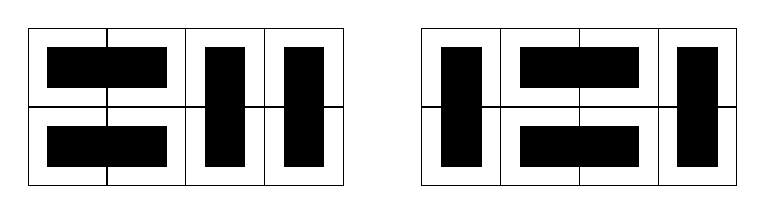
\begin{tikzpicture}[x=1.0cm, y=1.0cm]
        \foreach \y in {0,1} {
            \foreach \x in {0,...,3} {
                \draw (0+\x ,0+\y) rectangle ++ (1,1);
            }
        }

        \draw[fill, black] (0.25 ,0.25) rectangle ++ (1.5,0.5);
        \draw[fill, black] (0.25 ,1.25) rectangle ++ (1.5,0.5);
        \draw[fill, black] (2.25 ,0.25) rectangle ++ (0.5,1.5);
        \draw[fill, black] (3.25 ,0.25) rectangle ++ (0.5,1.5);

        \foreach \y in {0,1} {
            \foreach \x in {0,...,3} {
                \draw (5+\x ,0+\y) rectangle ++ (1,1);
            }
        }

        \draw[fill, black] (5+1.25 ,0.25) rectangle ++ (1.5,0.5);
        \draw[fill, black] (5+1.25 ,1.25) rectangle ++ (1.5,0.5);
        \draw[fill, black] (5+0.25 ,0.25) rectangle ++ (0.5,1.5);
        \draw[fill, black] (5+3.25 ,0.25) rectangle ++ (0.5,1.5);
    \end{tikzpicture}
\end{center}
而以下\emph{不}是正确的密铺

\begin{center}
    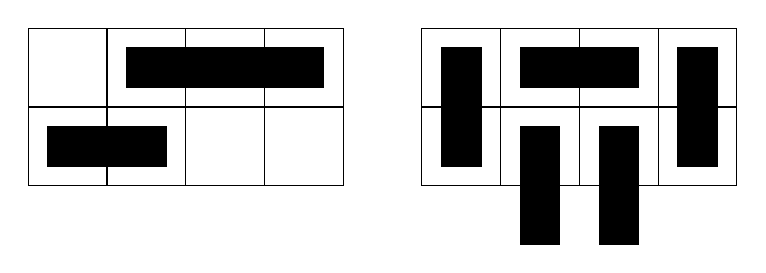
\begin{tikzpicture}[x=1.0cm, y=1.0cm]
        \foreach \y in {0,1} {
            \foreach \x in {0,...,3} {
                \draw (0+\x ,0+\y) rectangle ++ (1,1);
            }
        }

        \draw[fill, black] (0.25 ,0.25) rectangle ++ (1.5,0.5);
        \draw[fill, black] (1.25 ,1.25) rectangle ++ (1.5,0.5);
        \draw[fill, black] (2.25 ,1.25) rectangle ++ (1.5,0.5);

        \foreach \y in {0,1} {
            \foreach \x in {0,...,3} {
                \draw (5+\x ,0+\y) rectangle ++ (1,1);
            }
        }

        \draw[fill, black] (5+1.25 ,1.25) rectangle ++ (1.5,0.5);
        \draw[fill, black] (5+1.25 ,-0.75) rectangle ++ (0.5,1.5);
        \draw[fill, black] (5+2.25 ,-0.75) rectangle ++ (0.5,1.5);
        \draw[fill, black] (5+0.25 ,0.25) rectangle ++ (0.5,1.5);
        \draw[fill, black] (5+3.25 ,0.25) rectangle ++ (0.5,1.5);
    \end{tikzpicture}
\end{center}

和以前一样,让我们查看前几种情况(其中 $n = 1, 2, 3$ 等),看看我们是否能发现任何模式。在继续阅读之前,尝试自己解决该问题!

当 $n = 1$ 时,我们有一个与多米诺骨牌形状完全相同的棋盘,因此肯定只有一种方法可以密铺。让我们使用符号 $T(n)$ 来表示 $2 \times n$ 棋盘上的密铺数量。因此,$T(1) = 1$。

\begin{center}
    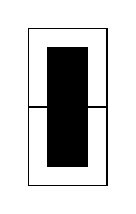
\begin{tikzpicture}[x=1.0cm, y=1.0cm]
        \draw (0,0) rectangle ++ (1,1);
        \draw (0,1) rectangle ++ (1,1);
        \draw[fill, black] (0.25 ,0.25) rectangle ++ (0.5,1.5);
    \end{tikzpicture}
\end{center}
当 $n = 2$ 时,我们有一个 $2 \times 2$ 棋盘。由于棋盘的方向很重要,因此我们有以下两种不同的密铺。因此,$T(2) = 2$。

\begin{center}
    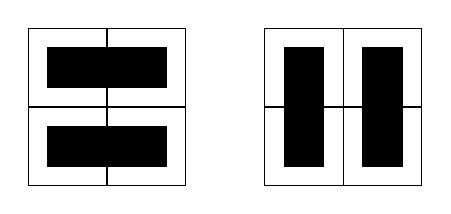
\begin{tikzpicture}[x=1.0cm, y=1.0cm]
        \foreach \y in {0,1} {
            \foreach \x in {0,1} {
                \draw (0+\x ,0+\y) rectangle ++ (1,1);
            }
        }

        \draw[fill, black] (0.25 ,0.25) rectangle ++ (1.5,0.5);
        \draw[fill, black] (0.25 ,1.25) rectangle ++ (1.5,0.5);

        \foreach \y in {0,1} {
            \foreach \x in {0,1} {
                \draw (3+\x ,0+\y) rectangle ++ (1,1);
            }
        }

        \draw[fill, black] (3+0.25 ,0.25) rectangle ++ (0.5,1.5);
        \draw[fill, black] (3+1.25 ,0.25) rectangle ++ (0.5,1.5);
    \end{tikzpicture}
\end{center}
当 $n = 3$ 时呢?同样地,我们可以手动枚举这些密铺,并确保没有遗漏任何一个。我们看到 $T(3) = 3$。

\begin{center}
    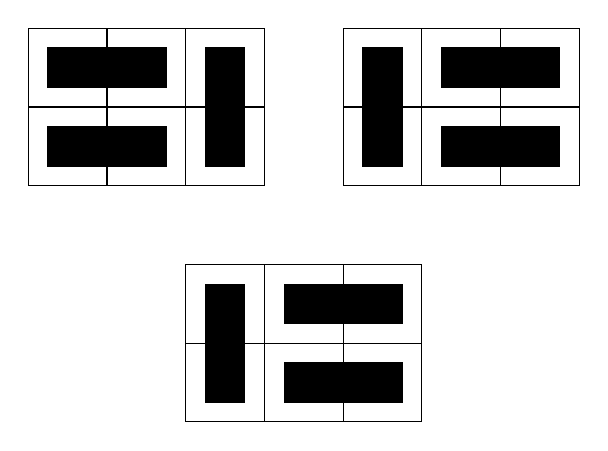
\begin{tikzpicture}[x=1.0cm, y=1.0cm]
        \foreach \y in {0,1} {
            \foreach \x in {0,1,2} {
                \draw (0+\x ,0+\y) rectangle ++ (1,1);
            }
        }

        \draw[fill, black] (0.25 ,0.25) rectangle ++ (1.5,0.5);
        \draw[fill, black] (0.25 ,1.25) rectangle ++ (1.5,0.5);
        \draw[fill, black] (2.25 ,0.25) rectangle ++ (0.5,1.5);

        \foreach \y in {0,1} {
            \foreach \x in {0,1,2} {
                \draw (4+\x ,0+\y) rectangle ++ (1,1);
            }
        }

        \draw[fill, black] (4+1.25 ,0.25) rectangle ++ (1.5,0.5);
        \draw[fill, black] (4+1.25 ,1.25) rectangle ++ (1.5,0.5);
        \draw[fill, black] (4+0.25 ,0.25) rectangle ++ (0.5,1.5);

        \foreach \y in {0,1} {
            \foreach \x in {0,1,2} {
                \draw (2+\x ,-3+\y) rectangle ++ (1,1);
            }
        }

        \draw[fill, black] (2+1.25 ,-3+0.25) rectangle ++ (1.5,0.5);
        \draw[fill, black] (2+1.25 ,-3+1.25) rectangle ++ (1.5,0.5);
        \draw[fill, black] (2+0.25 ,-3+0.25) rectangle ++ (0.5,1.5);
    \end{tikzpicture}
\end{center}
好的,再看一种情况,当 $n=4$ 时,我们看到 $T(4)=5$。

\begin{center}
    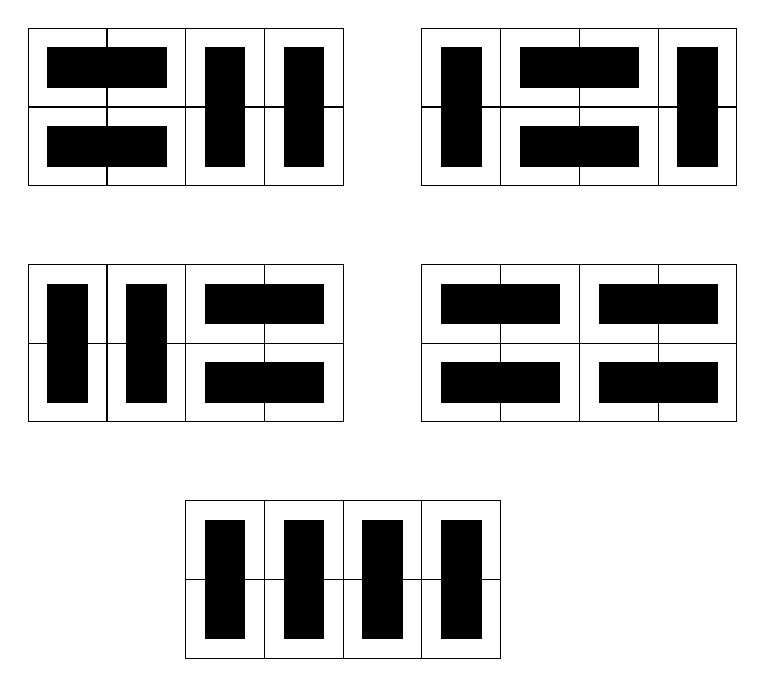
\begin{tikzpicture}[x=1.0cm, y=1.0cm]
        \foreach \y in {0,1} {
            \foreach \x in {0,...,3} {
                \draw (0+\x ,0+\y) rectangle ++ (1,1);
            }
        }

        \draw[fill, black] (0.25 ,0.25) rectangle ++ (1.5,0.5);
        \draw[fill, black] (0.25 ,1.25) rectangle ++ (1.5,0.5);
        \draw[fill, black] (2.25 ,0.25) rectangle ++ (0.5,1.5);
        \draw[fill, black] (3.25 ,0.25) rectangle ++ (0.5,1.5);

        \foreach \y in {0,1} {
            \foreach \x in {0,...,3} {
                \draw (5+\x ,0+\y) rectangle ++ (1,1);
            }
        }

        \draw[fill, black] (5+1.25 ,0.25) rectangle ++ (1.5,0.5);
        \draw[fill, black] (5+1.25 ,1.25) rectangle ++ (1.5,0.5);
        \draw[fill, black] (5+0.25 ,0.25) rectangle ++ (0.5,1.5);
        \draw[fill, black] (5+3.25 ,0.25) rectangle ++ (0.5,1.5);

        \foreach \y in {0,1} {
            \foreach \x in {0,...,3} {
                \draw (0+\x ,-3+\y) rectangle ++ (1,1);
            }
        }

        \draw[fill, black] (2.25 ,-3+0.25) rectangle ++ (1.5,0.5);
        \draw[fill, black] (2.25 ,-3+1.25) rectangle ++ (1.5,0.5);
        \draw[fill, black] (0.25 ,-3+0.25) rectangle ++ (0.5,1.5);
        \draw[fill, black] (1.25 ,-3+0.25) rectangle ++ (0.5,1.5);

        \foreach \y in {0,1} {
            \foreach \x in {0,...,3} {
                \draw (5+\x ,-3+\y) rectangle ++ (1,1);
            }
        }

        \draw[fill, black] (5+2.25 ,-3+0.25) rectangle ++ (1.5,0.5);
        \draw[fill, black] (5+2.25 ,-3+1.25) rectangle ++ (1.5,0.5);
        \draw[fill, black] (5+0.25 ,-3+0.25) rectangle ++ (1.5,0.5);
        \draw[fill, black] (5+0.25 ,-3+1.25) rectangle ++ (1.5,0.5);

        \foreach \y in {0,1} {
            \foreach \x in {0,...,3} {
                \draw (2+\x ,-6+\y) rectangle ++ (1,1);
            }
        }

        \draw[fill, black] (2+0.25 ,-6+0.25) rectangle ++ (0.5,1.5);
        \draw[fill, black] (2+1.25 ,-6+0.25) rectangle ++ (0.5,1.5);
        \draw[fill, black] (2+2.25 ,-6+0.25) rectangle ++ (0.5,1.5);
        \draw[fill, black] (2+3.25 ,-6+0.25) rectangle ++ (0.5,1.5);
    \end{tikzpicture}
\end{center}

我们现在可以开始寻找模式了吗?找到更大棋盘的密铺会很繁琐!让我们考虑一下如何利用 $T(1) = 1$ 的事实来推断出有关 $T(2)$ 的信息……等一下……做不到,对吧?这两个案例有本质的区别。具体来说,由于多米诺骨牌的大小为 $2 \times 1$,因此我们仅向棋盘中添加一行这一事实对我们没有帮助。

好吧,那么我们考虑 $n = 3$。我们可以利用 $T(2) = 2$ 这个事实吗?在这种情况下,答案是肯定的!知道 $2 \times 2$ 棋盘有两个密铺,无需太多思考,我们可以立即构建 $2 \times 3$ 棋盘的两个平铺。具体来说,我们可以将\emph{垂直多米诺骨牌添加}到之前的每一个密铺中。但我们知道 $T(3) = 3$。第三个密铺从何而来?再次查看该密铺,以及它与其他两个密铺的比较。在第三个密铺中,右侧的多米诺骨牌是水平的,而不是其他两种密铺中的垂直多米诺骨牌。如果我们移除这两个平行的水平多米诺骨牌,我们就会得到 $n = 1$ 时的情况。换句话说,我们可以通过在右侧\emph{添加一个由两个水平多米诺骨牌组成的正方形}来构建 $2 \times 3$ 棋盘的密铺。总的来说,我们已经用较小尺寸的棋盘(即 $2 \times 2$ 和 $2 \times 1$)描述了 $2 \times 3$ 棋盘的所有密铺:

\begin{center}
    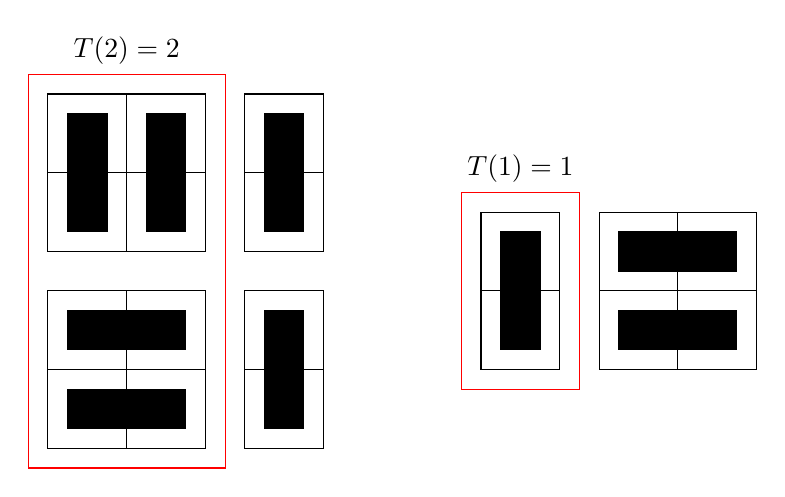
\begin{tikzpicture}[x=1.0cm, y=1.0cm]
        \foreach \g in {0, 2.5} {
            \foreach \y in {0,1} {
                \foreach \x in {0,1} {
                    \draw (0+\x ,0+\y+\g) rectangle ++ (1,1);
                }
            }
            \draw (2.5,0+\g) rectangle ++ (1,1);
            \draw (2.5,1+\g) rectangle ++ (1,1);
            \draw[fill, black] (2.75 ,0.25+\g) rectangle ++ (0.5,1.5);
        }

        \draw[fill, black] (0.25 ,0.25) rectangle ++ (1.5,0.5);
        \draw[fill, black] (0.25 ,1.25) rectangle ++ (1.5,0.5);

        \draw[fill, black] (0.25 ,2.5+0.25) rectangle ++ (0.5,1.5);
        \draw[fill, black] (1.25 ,2.5+0.25) rectangle ++ (0.5,1.5);

        \draw[red] (-0.25, -0.25) rectangle ++(2.5, 5);
        \path (-0.25,4.75) --  (2.25,4.75) node[midway,above,black] {$T(2)=2$};

        \draw (5.5,1) rectangle ++ (1,1);
        \draw (5.5,2) rectangle ++ (1,1);
        \draw[fill, black] (5.75 ,1.25) rectangle ++ (0.5,1.5);
        \draw[red] (5.25, 0.75) rectangle ++(1.5, 2.5);
        \path (5.25,3.25) --  (6.75,3.25) node[midway,above,black] {$T(1)=1$};

        \foreach \y in {0,1} {
            \foreach \x in {0,1} {
                \draw (7+\x ,1+\y) rectangle ++ (1,1);
            }
        }
        \draw[fill, black] (7.25 ,1.25) rectangle ++ (1.5,0.5);
        \draw[fill, black] (7.25 ,2.25) rectangle ++ (1.5,0.5);

    \end{tikzpicture}
\end{center}
\[T(3) = 3 = 2 + 1 = T(2) + T(1)\]

现在你可能会看出模式来!我们再看一下当 $n = 4$ 时会发生什么,我们将垂直多米诺骨牌添加到构成 $T(3)$ 的每一个密铺中,或者将两个水平多米诺骨牌添加到构成 $T(2)$ 的每一个密铺中,以此得到 $T(4)$ 的\emph{所有}密铺:

\begin{center}
    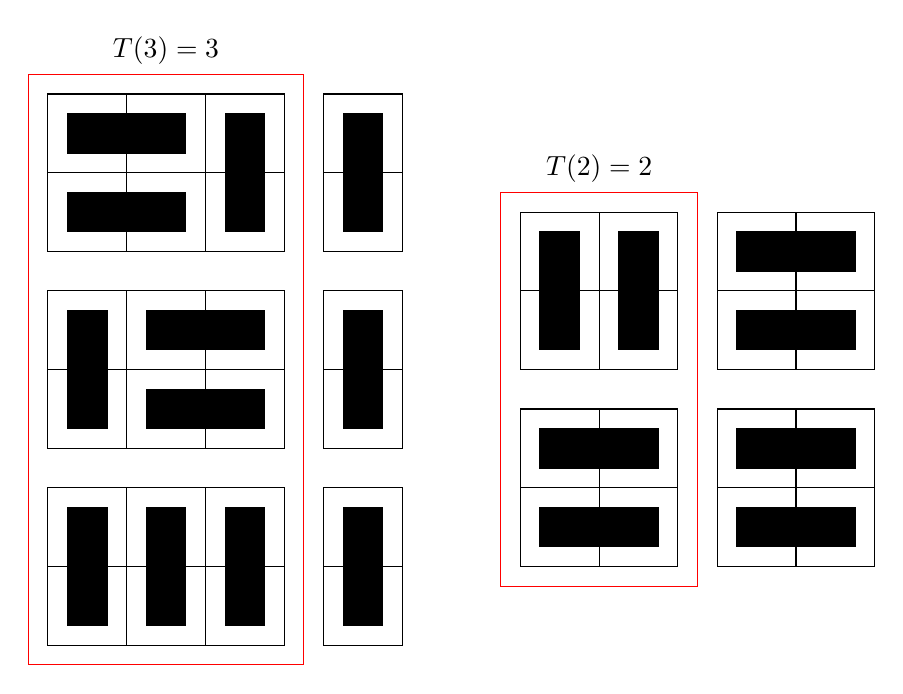
\begin{tikzpicture}[x=1.0cm, y=1.0cm]
        \foreach \g in {0, 2.5, 5} {
            \foreach \y in {0,1} {
                \foreach \x in {0,1,2} {
                    \draw (0+\x ,0+\y+\g) rectangle ++ (1,1);
                }
            }

            \draw (3.5,\g+0) rectangle ++ (1,1);
            \draw (3.5,\g+1) rectangle ++ (1,1);
            \draw[fill, black] (3.75 ,\g+0.25) rectangle ++ (0.5,1.5);
        }
        \draw[fill, black] (0.25 ,0.25) rectangle ++ (0.5,1.5);
        \draw[fill, black] (1.25 ,0.25) rectangle ++ (0.5,1.5);
        \draw[fill, black] (2.25 ,0.25) rectangle ++ (0.5,1.5);

        \draw[fill, black] (0.25 ,2.75) rectangle ++ (0.5,1.5);
        \draw[fill, black] (1.25 ,2.75) rectangle ++ (1.5,0.5);
        \draw[fill, black] (1.25 ,3.75) rectangle ++ (1.5,0.5);

        \draw[fill, black] (2.25 ,5.25) rectangle ++ (0.5,1.5);
        \draw[fill, black] (0.25 ,5.25) rectangle ++ (1.5,0.5);
        \draw[fill, black] (0.25 ,6.25) rectangle ++ (1.5,0.5);

        \draw[red] (-0.25, -0.25) rectangle ++(3.5, 7.5);
        \path (-0.25,7.25) --  (3.25,7.25) node[midway,above,black] {$T(3)=3$};


        \foreach \g in {0, 2.5} {
            \foreach \y in {0,1} {
                \foreach \x in {0,1} {
                    \draw (6+\x ,1+\y+\g) rectangle ++ (1,1);
                }
            }
            \foreach \y in {0,1} {
                \foreach \x in {0,1} {
                    \draw (8.5+\x ,1+\y+\g) rectangle ++ (1,1);
                }
                \draw[fill, black] (8.75 ,1.25+\g+\y) rectangle ++ (1.5,0.5);
            }
           
        }

        \draw[fill, black] (6.25 ,1.25) rectangle ++ (1.5,0.5);
        \draw[fill, black] (6.25 ,2.25) rectangle ++ (1.5,0.5);

        \draw[fill, black] (6.25 ,3.5+0.25) rectangle ++ (0.5,1.5);
        \draw[fill, black] (7.25 ,3.5+0.25) rectangle ++ (0.5,1.5);

        \draw[red] (5.75, 0.75) rectangle ++(2.5, 5);
        \path (5.75,5.75) --  (8.25,5.75) node[midway,above,black] {$T(2)=2$};
        
    \end{tikzpicture}
\end{center}
\[T(4) = 5 = 3 + 2 = T(3) + T(2)\]

另请注意,用这种方式不会产生重复的 $2 \times 4$ 密铺。(仔细想想为什么会这样。我们用一种什么方法表征两种密铺可以保证它们不重复?)有了这些信息,我们可以立即得出结论 $T(4) = T(3) + T(2)$。

此外,我们可以概括这样一个论点;$n = 4$ 没有什么特别的,对吧?对于任意特定的 $n$,我们可以只考虑所有可能的密铺,然后看看棋盘\emph{最右侧}发生的情况:要么有一个垂直多米诺骨牌(这意味着密铺来自 $2 \times (n - 1)$ 棋盘),要么有两个水平多米诺骨牌(这意味着密铺来自 $2 \times (n-2)$ 棋盘)。有了这个论点的支撑,对于所有有意义的 $n$ 值,我们可以得出如下结论:
\[T(n) = T(n - 1) + T(n - 2)\]
哪些 $n$ 值有意义?请记住,我们必须单独分析 $T(1)$ 和 $T(2)$;因此这个论点不适用于 $n=1$ 和 $n=2$,我们必须添加限制条件 $n \ge 3$ 才能使上面公式成立。

有了这些信息,只要有足够的时间,我们就可以轻松计算出任意 $n$ 值下的 $T(n)$。我们甚至可以相当容易地编写出计算机程序。然而,正是这种\emph{归纳}论证——我们注意到的模式以及我们对其发生原因的彻底描述——让我们首先得出了结论。这种情况下,每一项的值 $T(n)$ 取决于前\emph{两}项 $T(n-1)$ 和 $T(n-2)$ 的值。这在本章之前的例子中\emph{没有}出现过,它暗示了这里发生了更深层次的事情。你是否发现我们之前对归纳的定义以及多米诺骨牌的类比在这里不再适用?你会如何修正我们的类比来解释这种情况?思考一下这些问题,然后继续阅读。我们将在下一个示例之后更深入地讨论它们。

顺便一提,你是否注意到此示例的解有一些有趣的地方?你还知道其他类似的数列吗?想一想……

\subsection{制胜策略}

这个例子将是我们第一个\emph{无需}证明数值公式的归纳问题!这似乎很奇怪,但正如即将看到的那样,这却是一个事实。实际上在数学中,这比你想象的更常见:一个问题或数学对象可能存在某些潜在的归纳结构,但却不依赖代数或算术的内容。

事实上,我们将讨论一个\emph{游戏}。就是通常意义上的游戏——有两个玩家必须遵守的规则,并且有明显的赢家和输家——同时也是数学意义上的游戏,我们可以使用数学符号来制定规则和游戏情境,并以抽象的方式讨论\emph{策略}。我们甚至可以\emph{解}这个游戏。这与棒球比赛非常不同。

现在让我们讨论一下这个游戏的规则,我们暂时将其称为``取石子''。有两个玩家,称为 $P_1$ 和 $P_2$。玩家 $P_1$ 先行。玩家面前的桌子上有两堆石子,每堆正好有 $n$ 个石子,其中 $n$ 是某个自然数。(为了区分游戏的不同版本,当每堆石子有 $n$ 个石子时,我们会说玩家正在``玩 $T_n$''。)在每个玩家的回合中,他们可以从\emph{任意}一堆中取走\emph{任意}数量的石子。但不能同时从两堆石子中取石子。取走\emph{最后}一颗石子的玩家\emph{获胜}。

试着跟朋友玩一下这个游戏。使用硬币或糖果当石子。再试着切换一下角色,你先作为 $P_1$,然后再作为 $P_2$。尝试制定一个获胜\emph{策略},一种最大化获胜机会的游戏方法。尝试猜测不同的 $n$ 值下会发生什么。谁``应该''获胜?你能\emph{证明}吗?说真的,在继续阅读我们的分析之前,先玩玩这个游戏并尝试证明一些结论。你可能会对自己所取得的成就感到惊讶!

与其他示例一样,让我们使用 $n$ 的一些较小值来弄清楚到底发生了什么,然后再尝试进行泛化。当 $n = 1$ 时,这个游戏相当愚蠢。$P_1$ 必须取走其中一堆中唯一的石子,然后 $P_2$ 取走另一堆中唯一剩余的石子。因此,$P_2$ 胜。(请注意,无论 $P_1$ 选择两堆中的哪一堆,$P_2$ 总是会得到另一堆。我们可以说``不失一般性'', $P_1$ 选择左边这堆,因为无论选择哪一堆都无关紧要;情况是等价的,所以为了方便具体讨论,我们不妨说是左边这堆。后面讨论数理逻辑时,我们也会深入探讨``不失一般性''这一思想。)


\begin{center}
    \begin{tikzpicture}[line width=0.5mm]
        \foreach \n in {0, 1}{
            \node at (\n, 0)[circle,fill,inner sep=8pt, anchor=west]{};
            \draw (\n, -1) -- +(0.8, 0);
        }
        \draw[-latex] (2.5, -0.4) -- +(2, 0) node[midway,above]{$P_1$ 回合};
        \draw (5, -1) -- +(0.8, 0);
        \node at (6, 0)[circle,fill,inner sep=8pt, anchor=west]{};
        \draw (6, -1) -- +(0.8, 0);
        \draw[-latex] (7.5, -0.4) -- +(2, 0) node[midway,above]{$P_2$ 回合};
        \draw (10, -1) -- +(0.8, 0);
        \draw (11, -1) -- +(0.8, 0);
        \path (10, -0.4) -- +(2, 0) node[midway,above]{$P_2$ 胜!};
    \end{tikzpicture}
\end{center}

当 $n = 2$ 时,可能会出现几种情况。思考 $P_1$ 可能采取的行动。同样地,$P_1$ 可能选择左堆也可能选择右堆,但因为最终结果是相同的,并且我们可以交换这两堆,所以我们可以说(不失一般性)$P_1$ 从左堆取走若干石子。具体是多少?可能是一颗石子也可能是两颗石子。让我们分别检验每种情况。

\begin{center}
    \begin{tikzpicture}[line width=0.5mm]
        \foreach \x in {0, 1}{
            \node at (\x, 0)[circle,fill,inner sep=8pt, anchor=west]{};
            \node at (\x, 1)[circle,fill,inner sep=8pt, anchor=west]{};
            \draw (\x, -1) -- +(0.8, 0);
        }
        \draw[-latex] (2.5, -0.4) -- +(2, -0.6);
        \draw[-latex] (2.5, 0.6) -- +(2, 0.6);
        \node[anchor=west] at(2.5,0) {$P_1$ 回合};
        \foreach \delta in {1, -2}{
            \foreach \n in {0, 1}{
                \draw (5+\n, \delta) -- +(0.8, 0);
                \node at (6, \delta+1+\n)[circle,fill,inner sep=8pt, anchor=west]{};
            }
        }
        \node at (5, -1)[circle,fill,inner sep=8pt, anchor=west]{};
        \draw[-latex] (7.5, 2) -- +(2, 0) node[midway,above]{$P_2$ 回合};
        \draw[-latex] (7.5, -1) -- +(2, 0) node[midway,above]{$P_2$ 回合};
        \draw (10, 1) -- +(0.8, 0);
        \draw (11, 1) -- +(0.8, 0);
        \path (10, 1.6) -- +(2, 0) node[midway,above]{$P_2$ 胜!};
        \path (10, -1.4) -- +(2, 0) node[midway,above]{???};
    \end{tikzpicture}
\end{center}

如果 $P_1$ 取走两颗石子,$P_2$ 应该如何应对呢?$P_2$ 可以取走另一堆从而获胜,所以 $P_1$ 一开始就不应该采取这一行动。不过,可能 $P_1$ 脑子不清什么的,而且我们需要考虑所有可能的情况来全面分析这场比赛。因此,在这种情况下(上图中的上半行)$P_2$ 获胜。好吧,这就是简单的情况。

如果 $P_1$ 只从左边一堆石子(上图中的下半行)中取走一颗石子怎么办?$P_2$ 应该如何应对?我们现在有几种选择:

\begin{itemize}
    \item 如果 $P_2$ 从左边一堆石子中取走另一颗石子……那么,$P_2$ 取走另一堆全部石子,$P_1$ 获胜。
    \item 如果 $P_2$ 从右边一堆石子中取走全部两颗石子……那么,$P_1$ 取走左边一堆中的最后一颗石子,$P_1$ 获胜。
    \item 然而,如果 $P_2$ 只从右边一堆石子中取走一颗石子……
\end{itemize}

\begin{center}
    \begin{tikzpicture}[line width=0.5mm]
        \foreach \g in {0, 5, 10} {
            \foreach \x in {0, 1} {
                \node at (\x+\g, 0)[circle,fill,inner sep=8pt, anchor=west]{};
                \draw (\x+\g, -1) -- +(0.8, 0);
            }
        }
        \node at (0, 1)[circle,fill,inner sep=8pt, anchor=west]{};
        \node at (1, 1)[circle,fill,inner sep=8pt, anchor=west]{};
        \draw[-latex] (2.5, -0.4) -- +(2, 0) node[midway,above]{$P_1$ 回合};

        \node at (6, 1)[circle,fill,inner sep=8pt, anchor=west]{};
        \draw[-latex] (7.5, -0.4) -- +(2, 0) node[midway,above]{$P_2$ 回合};
    \end{tikzpicture}
\end{center}
现在我们遇到了与 $T_1$ 完全相同的情况,我们已经对此进行了分析!这次又是 $P_1$ 先走的,所以我们知道会发生什么:无论如何 $P_2$ 都会获胜。如果你是玩家 $P_2$,这显然是最好的应对:\emph{无论} $P_1$ \emph{如何行动},你都会赢!

退一步,让我们思考一下这表明了什么:无论 $P_1$ 首先采取什么行动(从任一堆中取走一个或两个石子),$P_2$ 都可以做出\emph{某个可能的回应,保证} $P_2$ 总会获胜,无论 $P_1$ 随后采取什么回应。哇,$P_2$ 稳坐钓鱼台!让我们看看其他 $n$ 值的情况下是否会发生同样的事情。

当 $n = 3$ 时,我们将再次假设(不失一般性)玩家 $P_1$ 从左边石子堆上取石子。他可以取走一颗、两颗或三颗石子:

\begin{itemize}
    \item 如果 $P_1$ 取走全部三颗,那么 $P_2$ 就会完全拿走另一堆并获胜。
    \item 如果 $P_1$ 取走两颗石子……那么 $P_2$ 应该做什么呢?
\end{itemize}
取完左边一堆是愚蠢的(因为 $P_1$ 可以取走整个右边一堆从而获胜),而取走整个右边一堆也同样愚蠢(因为 $P_1$ 可以取走整个左边一堆从而获胜),所以需要介于两者之间。现在,如果 $P_2$ 仅从右侧一堆石子中取走一颗石子,请注意 $P_1$ 可以采用相同的动作做出回应;从而使得两堆石子都只剩下一颗,但先手互换了。在这种情况下,$P_2$ 先行,根据我们之前的分析,$P_2$ 肯定会输。因此这是糟糕的策略!

\begin{center}
    \begin{tikzpicture}[line width=0.5mm]
        \foreach \g in {0, 5, 10, 15}{
            \foreach \x in {0, 1}{
                \node at (\x+\g, 0)[circle,fill,inner sep=8pt, anchor=west]{};
                \draw (\x+\g, -1) -- +(0.8, 0);
            }
        }
        \foreach \x in {0, 1, 6}{
            \foreach \y in {0, 1}{
                \node at (\x, \y)[circle,fill,inner sep=8pt, anchor=west]{};
                \node at (\x, \y+1)[circle,fill,inner sep=8pt, anchor=west]{};
            }
        }

        \node at (11, 1)[circle,fill,inner sep=8pt, anchor=west]{};

        \draw[-latex] (2.5, -0.4) -- +(2, 0) node[midway,above]{$P_1$ 回合};
        \draw[-latex] (7.5, -0.4) -- +(2, 0) node[midway,above]{$P_2$ 回合};
        \draw[-latex] (12.5, -0.4) -- +(2, 0) node[midway,above]{$P_1$ 回合};
        \path (15, 0.6) -- +(2, 0) node[midway,above]{$P_1$ 胜!};
    \end{tikzpicture}
\end{center}

让我们再试一次。如果 $P_2$ 从右边一堆石子中取走两颗石子……瞧!现在,我们每堆中只有一颗石子,$P_1$ 先行,所以我们知道  $P_1$ 一定会输。$P_2$ 再次完胜!

\begin{center}
    \begin{tikzpicture}[line width=0.5mm]
        \foreach \g in {0, 5, 10}{
            \foreach \x in {0, 1}{
                \node at (\x+\g, 0)[circle,fill,inner sep=8pt, anchor=west]{};
                \draw (\x+\g, -1) -- +(0.8, 0);
            }
        }
        \foreach \x in {0, 1, 6}{
            \foreach \y in {0, 1}{
                \node at (\x, \y)[circle,fill,inner sep=8pt, anchor=west]{};
            }
        }
        \draw[-latex] (2.5, -0.4) -- +(2, 0) node[midway,above]{$P_1$ 回合};
        \draw[-latex] (7.5, -0.4) -- +(2, 0) node[midway,above]{$P_2$ 回合};
        \path (10, 0.6) -- +(2, 0) node[midway,above]{$P_2$ 胜!};
    \end{tikzpicture}
\end{center}

思考一下 $n = 4$ 的情况,你会发现完全相同的分析再次出现。你会考虑另一种可能性:玩家 $P_1$ 可以从左边一堆石子中取走一颗、两颗、三颗或四颗。不过,无论 $P_1$ 怎么做,你都会发现 $P_2$ 可以在另一堆上\emph{模仿}相同的动作,将整个游戏简化为之前的\emph{较小}版本,从而保证 $P_2$ 一定获胜!看起来 $P_2$ 一直处于主导地位,因为他可以对 $P_1$ 的任何行为做出回应,在另一堆上做出相同的动作。无论 $P_1$ 做什么,$P_2$ 总会做出回应,这意味着 $P_2$ 一定获胜,无论 $P_1$ 随后的动作是什么。从这个意义上讲,我们说``$P_2$ 有制胜策略''。$P_2$ 有一个清晰且可描述的方法来评估比赛局势并选择特定的行动来\emph{保证获胜}。

我们要如何证明这一点?如何应用本章的归纳法?目前可能很难看出来。我们在这里到底要证明什么?对这个问题的类比中,多米诺骨牌或阶梯是什么?在你开动脑筋思考这个例子时,你应该意识到以下几点:归纳法并不总是与代数式有关;归纳法代表某种``构建''结构,较大的情况依赖于较小的情况;我们必须证明一些初始事实,然后论证如何化简任意更大事实,使其依赖于先前的事实。这才是多米诺骨牌类比的真正目的。碰巧的是,这个类比可以很好地解释某些归纳问题(但不是全部),并且是可视化的,令人印象深刻。但它并不完全适用于\emph{所有}情况。

回顾本章的四个例子,思考它们有何相似之处和不同之处。 尝试使用一些更好的术语(也许是你自己发明的)对数学归纳法进行更精确的数学描述。(这里的意思是比直观的类比更好。你会惊讶地发现,在不真正知道自己``应该''说什么的情况下,你竟然能够很好地描述归纳法,并且在这个过程中你会学到很多东西!)在适当的时候,我们会对数学归纳法及其各种形式进行严格的陈述和证明。与此同时,我们需要探索数学的一些其他领域,以建立必要的语言、符号和知识,以便回过头解决这个问题。不过,在开始之前,我们应该了解一下数学归纳法的一些有用的应用。

\subsection{习题}

\subsubsection*{温故知新}

以口头或书面的形式简要回答以下问题。这些问题全都基于你刚刚阅读的内容,所以如果忘记了具体的定义、概念或示例,可以回去重读相关部分。确保在继续学习之前能够自信地回答这些问题,这将有助于你的理解和记忆!

\begin{enumerate}[label=(\arabic*)]
    \item 这两个例子如何\emph{归纳}?它们在哪些方面与前面的例子(立方体和直线)相似?哪些方面有所不同?
    \item 对于多米诺骨牌密铺问题,我们需要知道多少个先前值才能计算 $T(n)$?
    \item $T(n) = T(n - 1) + T(n - 2)$ 和 $T(n + 2) = T(n + 1) + T(n)$ 有什么区别?
    \item 取石子游戏的必胜策略是什么?尝试与一个不了解该游戏的朋友一起玩一下,并使用玩家 $P_2$ 的必胜策略。每次你都获胜时他们有多沮丧?他们也开始发现这个策略了吗?
\end{enumerate}

\subsubsection*{小试牛刀}

尝试回答以下问题。这些题目要求你实际动笔写下答案,或(对朋友/同学)口头陈述答案。目的是帮助你练习使用新的概念、定义和符号。题目都比较简单,确保能够解决这些问题将对你大有帮助!

\begin{enumerate}[label=(\arabic*)]
    \item $T(5)$ 会是怎样?你能画出所有密铺方案吗?
    \item 探讨用两堆各 $4$ 颗石子进行取石子游戏的可能性。你能确保玩家 $P_2$ 总是有必胜策略吗?
    \item \textbf{挑战题:}如果用\emph{三堆}相同大小的石子来玩``取石子''游戏,会发生什么?你能为任意一方找到获胜策略吗?尝试和朋友一起玩一下,看看会发生什么!
    \item 查看\emph{斐波那契数列}。它与我们在多米诺骨牌密铺示例中发现的数列 $T(n)$ 有什么关系?
\end{enumerate}